\section{Overview of analysis}\label{sec:analysis}
%Mention the two steps. Dataflow analysis step. and then the escape analysis step.
%Insert a pseudocode snippet
For the scope of ECE750, only the intra-procedural analysis of the complete program analysis is completed. This mean that, for this project, the functionality of the program is only limited to doing intra-procedural analysis on a given method to detect whether an immutable local variable or a field reference escapes at a certain program point in a method, and checks whether a variable with the same \textit{Object Representative} is used at a later program point. If such a case does happen, then because of the use case of the immutable object in the respective method, the object cannot be transformed to mutable. Firstly, this section explains the intra procedural dataflow analysis that happens in the program. Secondly, it explains the reason for the usage of Object Representatives \cite{ref:or} in the scope of the data flow analysis. Lastly the escape analysis rules used in the project to detect object escaping is explained. The intra-procedural analysis is done using the dataflow analysis API provided by the Soot framework \citep{ref:Soot}.

\subsection{Dataflow Analysis}\label{sec:dataflow}
The dataflow analysis is a ``may-alias'' forward analysis, where each unit in the analysis graph stores a HashMap of the local variables or field references and their object representatives at the respective program point. Each of the design choices for the data flow analysis are explained below.

\textbf{Direction of Analysis:} The direction of the analysis is chosen to be forward analysis because in each step of the flow through function, the information about the variables in previous program points is of interest to subsequent program points. This is important because in the escape analysis step of the algorithm followed by the dataflow analysis step, the object representatives mapping of the variable from previous program points is used to determine whether it is safe to make the object immutable or not.

%Flowthrough with Object Representative
\textbf{Flowthrough Reaching Condition:} The reaching condition for the flowthrough of information in a unit done according to the following rules. Each unit of the analysis graph stores a HashMap that stores an instance of the Local variable of a field reference along with its Object Representative that is generated along the flowthrough function.
\vspace{5mm}

\begin{algorithm}
\caption{Flowthrough algorithm for dataflow analysis}
\label{fig:flowthrough}
\begin{algorithmic}
  \State Copy InSet to OutSet\;
  \If{Stmt is DefinitionStmt}
	\If{rhs is LocalVariable}
		\State OutSet.put(lhs, rhs.ObjectRep)\;
	\Else
		\State generateObjectRep\;
		\State OutSet.put(lhs, newObjectRep)\;
	\EndIf	

  \EndIf
\end{algorithmic}
\end{algorithm}
%Mayalias(merge)
\textbf{Merge Condition: } The merge condition for this analysis is done in the form of May-Analysis, because a variable may attain different ObjectRepresentatives in different branches. In that case, both the object representative for the object are stored with respect to the program point in which the merge is happening. This is necessary because if the object escapes within the branch, and in a subsequent program pointer if either of the Object Representatives aliases with a variable being used in the Stmt, then the object is still considered to be non-transformable to mutable because the used object ``may'' have escaped in a branch. This is a may-analysis because information about both the branches are recorded for analysis rather a definitive must analysis where the same condition must hold for both branches.

\subsection{Object Representatives}\label{sec:OR}
%Talk about what is object representative (Cite)
In this analysis Object Representatives need to be used because in this analysis objects aliasing with respect to their pointers to the heap are of interest rather than their value assignments in the stack. Generally in order to infer object reference to the heap, an inter-procedural analysis is necessary. However object representatives are a technique of dereferencing heap pointers to local objects from within an intra-procedural analysis \cite{ref:or}.

This is evident in our analysis of the client with the escaping object shown previously in figure \ref{fig:client_escape}. In that example, the escaped instance of \texttt{a} would have the same object representative as the field \texttt{escaper}, that is called later in the program although they were assigned to the heap in a seperate method from the subject method. If instead, an integer value assignment for the object instance and the field was used during the dataflow analysis, then this analysis would not be possible because they would have different value assignments. Without dereferencing pointers to the heap there is no way for programs to do this aliasing without using object representatives.
%Talk about why object representative is needed.
%How it is applied in this regard

\subsection{EscapeAnalysis}\label{sec:escape}
%Introduce the concept from the paper (cite)
In this program, escape analysis is used to detect objects that are escaping the stack to the heap, which causes objects to be globally accessible and hence prevent tranformation. There has been much work centered around escape analysis in the last decade, most of which has been towards its application in creating thread safe programs and optimizing multithreaded programming. The papers by Choi et al. and Vivien et. al \cite{ref:escapejava}\cite{ref:incrementalescape} were some of the first papers to introduce the escape analysis in the context of inter-procedural analysis. Both the papers were focused on the application of escape analysis to minimize object allocation to the heap with the objective of reducing sychronization operation for threads.

Surprisingly, escape analysis is seldom used in the context of intraprocedural analysis. The only work that relates to this project with respect to escape analysis is its application in dynamic compilation and deoptimization \cite{ref:globalescape} which uses escape analysis both in the context of intraprocedural analysis interprocedural analysis. Much of the intraprocedural inference techniques used in this work has been inspired by the works presented there.

%Talk about the rules with respect to this analysis (one paragraph each)
There are many programming use cases which causes local objects inside methods to escape the stack and get allocated to the heap, however in the scope of this research only some rules apply to the analysis. The applicable rules of escape analysis that apply in this context are strictly those related to object instance sharing and accessibility. According to existing research \cite{ref:globalescape} there are two categories of object escaping: \textit{global escape} \& \textit{method escape}. In the context of this research only the global escape of objects is relevant. Objects that suffer from method escape are also called \textit{thread-local} objects which means that the object has escaped the context of the method, but is local with respect to the thread running the method. Since the focus of this analysis is not to optimize synchronization calls with respect to threading, this type of object escape not relavant for this analysis.

The cases of \textit{global escape} relevant to this research is listed below:

\texttt{T.sf = a :} A local variable escapes its local allocation on the stack to the heap when it is assigned to a static field of the class. Being assigned to the static field of a class allows the object instance to be referenced by multiple methods and that is causes the object to escape. In terms of static analysis, this can checked trivially by checking that the left operand is a member of the field deference list, and that it of type \texttt{static}, then checking that the right operand is a local variable, in which case the assignee is the variable escaping ie.\ \texttt{a}.

\texttt{p.f = a :} When local variable is assigned to the field of another local variable, the assigned local variable is defined as escaped. The reason for this is that, if the assignee is mutable, and it is assigned to field of another local variable, any changes to the field of the local variable will cause the assigned variable to be changed as well. This is shown in the sample code segment in figure \ref{fig:fieldassignment}.

\begin{figure}[H]
	\caption{Object escape with local field assignment} \label{fig:fieldassignment}
	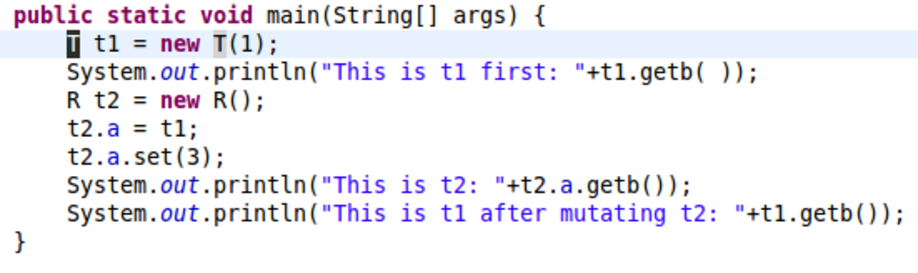
\includegraphics[width=0.5\textwidth]{img/fieldassignmentcod}
	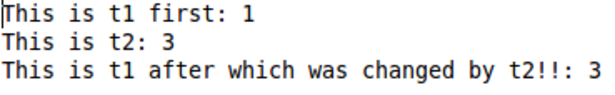
\includegraphics[width=0.3\textwidth]{img/fieldassignmentresult}
\end{figure}

In figure \ref{fig:fieldassignment} two local variable objects \texttt{t1} and \texttt{t2} are created, where \texttt{t2} owns an attribute with the same type as \texttt{t1} where \texttt{t1} is mutable. \texttt{t1} is assigned to the field \texttt{a} of t2 and followed by that the field of \texttt{t2} is mutated. After the mutation, it is seen from the output that due to the change in the field of \texttt{t2} the original variable also gets changed. It is difficult to resolve this aliasing in the dataflow analysis because the dataflow analysis only stores the object representatives of the local variables, but it does not store the object representatives of the fields of the local variables. Therefore, it is conservatively assumed in this analysis that whenever a local is assigned to the field of another variable, the assignee is marked as ``escaped'' irrespective of whether the field of the local variable actually gets mutated or not. This could have been avoided if the implementation of the type of \texttt{t1} was immutable, so that the \texttt{set()} method of object returned a new instance of the object, rather mutating the existing attribute.
%put an algorithm snippet if possible

\texttt{foo(a) :} A local variable is declared as escaped when it is passed as a parameter to another method. The reason for this is that the calling method could possibly mutate the object. From just intra procedural analysis it is impossible to know whether the calling method will actually mutate the object or not, and therefore for this analysis it is conservatively assumed that when an object is passed as a parameter to another method it has escaped the stack and is therefore deemed as escaped. Ideally it would be possible to check the operations on the passed in variable through an interprocedural analysis where one can transitively analyze whether any of the pointers of the object are being mutated by the calling methods. However, the inter-procedure analysis is beyond the scope of this project and is therefore a possible candidate for future work. This case of \textit{global escape} is being exhibitted in figure \ref{fig:client_escape} in section \ref{sec:example}. In that example, the local variable was being passed as a parameter to the method \texttt{escape()} and therefore at that program point that specific instace of the variable \texttt{a} is flagged as ``escaped''.

